\section{Anwendungen}
\begin{frame}{Anwendungen}
	\begin{itemize}
		\item Analyse neuraler Netzwerke
				\only<1>{\\ \ \\ \ \\ 
					\colorbox{YellowGreen}{Diagnose von Parkinson}}
		\item Zucht von Mikroorganismen
				\only<2>{\\ \ \\ \ \\ 
					\colorbox{YellowGreen}{Zusammensetzung der Nährstoffe}}
		\item Objektlageerkennung in Tiefendaten	
	\end{itemize}
\end{frame}

\begin{frame}{Anwendungen}
	\begin{itemize}
		\item Ausgangslage
				\only<1>{
					\begin{figure}
						\begin{minipage}{4.5cm}
							\centering
							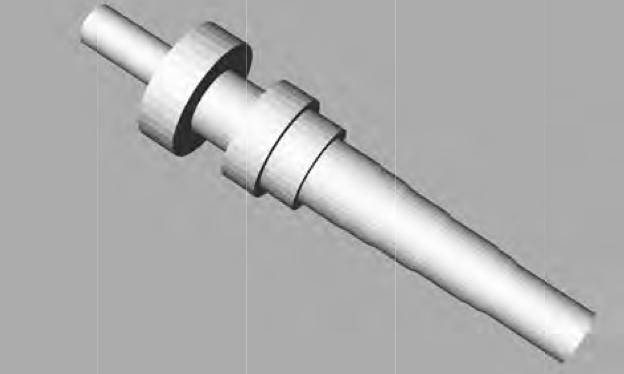
\includegraphics[width=4cm]{Bilder/welle-cad} \\
							CAD-Modell einer Getriebewelle
						\end{minipage}
						\begin{minipage}{4.5cm}
							\centering
							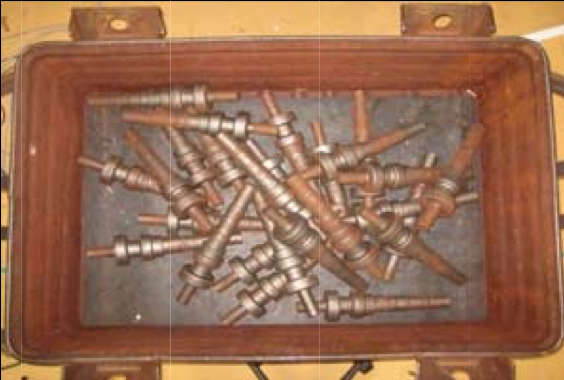
\includegraphics[width=4cm]{Bilder/welle-kiste} \\
							Beispiel einer Kiste mit Getriebewellen zur Ultraschallprüfung
						\end{minipage}
					\end{figure}
				}
		\item Objektorientierung $R_i$	
			\only<2>{
				\begin{figure}
					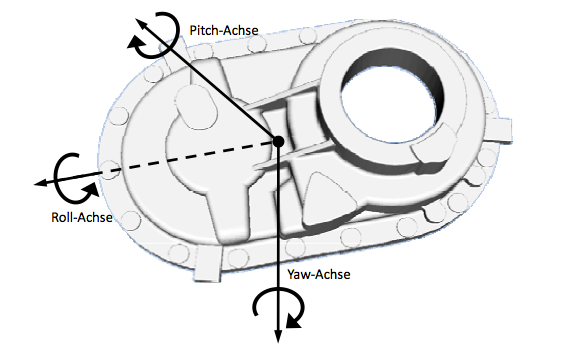
\includegraphics[width=5cm]{Bilder/yaw-pitch-roll}
				\end{figure}
			}
		\item Objektposition $P_i$
			\only<3>{\\ \ \\ 
				\colorbox{YellowGreen}{Referenzpunkt: höchster Punkt}}
		\item Objektmerkmalsdaten $C_i$
			\only<4>{\\ \ \\ 
				\colorbox{YellowGreen}{Segmentierung der Tiefendaten}}
		\item Fitnessfunktion: $f(p_i) = f(R_i,P_i,C_i)$
			\only<5>{\\ \ \\
				\colorbox{YellowGreen}{Vergleich mit Histogrammen aus Wissensbasis}}
		\item Schwarm
			\only<6>{\\ \ \\
				\colorbox{YellowGreen}{100 Partikel, lbest mit 30 Nachbarn, 100 Iterationen}}
		\item Resultat
			\only<7>{\\ \ \\
				\colorbox{YellowGreen}{Dauer: 4s, Erkennungsrate $>92\%$}}
	\end{itemize}
\end{frame}